\ifx\allfiles\undefined
\documentclass[12pt, a4paper, oneside, UTF8]{ctexbook}
\def\path{../config}
\usepackage{amsmath}
\usepackage{amsthm}
\usepackage{amssymb}
\usepackage{graphicx}
\usepackage{mathrsfs}
\usepackage{enumitem}
\usepackage{geometry}
\usepackage[colorlinks, linkcolor=black]{hyperref}
\usepackage{stackengine}
\usepackage{yhmath}
\usepackage{extarrows}

\usepackage{multicol}
\usepackage{fancyhdr}
\usepackage[dvipsnames, svgnames]{xcolor}
\usepackage{listings}
\usepackage{subfigure}
\usepackage{tikz}


\definecolor{mygreen}{rgb}{0,0.6,0}
\definecolor{mygray}{rgb}{0.5,0.5,0.5}
\definecolor{mymauve}{rgb}{0.58,0,0.82}

\graphicspath{ {figure/},{../figure/}, {config/}, {../config/} }

\linespread{1.6}

\geometry{
    top=25.4mm, 
    bottom=25.4mm, 
    left=20mm, 
    right=20mm, 
    headheight=2.17cm, 
    headsep=4mm, 
    footskip=12mm
}

\setenumerate[1]{itemsep=5pt,partopsep=0pt,parsep=\parskip,topsep=5pt}
\setitemize[1]{itemsep=5pt,partopsep=0pt,parsep=\parskip,topsep=5pt}
\setdescription{leftmargin=4em,itemsep=5pt,partopsep=0pt,parsep=\parskip,topsep=5pt}

\lstset{
    language=Mathematica,
    basicstyle=\tt,
    breaklines=true,
    keywordstyle=\bfseries\color{NavyBlue}, 
    emphstyle=\bfseries\color{Rhodamine},
    commentstyle=\itshape\color{black!50!white}, 
    stringstyle=\bfseries\color{PineGreen!90!black},
    columns=flexible,
    numbers=left,
    numberstyle=\footnotesize,
    frame=tb,
    breakatwhitespace=false,
} 
% 定理环境
\usepackage{tcolorbox}
\tcbuselibrary{most}
\theoremstyle{definition}


\newtheorem{proposition}{\indent 命题}[section]
\newtheorem{example}{\indent \color{SeaGreen}{例}}[section]
\theoremstyle{plain}
\newtheorem*{rmk}{\indent 注}
\renewenvironment{proof}{\indent\textcolor{SkyBlue}{\textbf{证明.}}\;}{\qed\par}
\newenvironment{solution}{\indent\textcolor{SkyBlue}{\textbf{解.}}\;}{\qed\par}
% #### 将 config.tex 中的定理环境的对应部分替换为如下内容
% 定义单独编号,其他四个共用一个编号计数 这里只列举了五种,其他可类似定义(未定义的使用原来的也可)
\newtcbtheorem[number within=section]{defn}%
{定义}{colback=OliveGreen!10,colframe=Green!70,fonttitle=\bfseries}{def}

\newtcbtheorem[number within=section]{lemma}%
{引理}{colback=Salmon!20,colframe=Salmon!90!Black,fonttitle=\bfseries}{lem}

% 使用另一个计数器 use counter from=lemma
\newtcbtheorem[use counter from=lemma, number within=section]{them}%
{定理}{colback=SeaGreen!10!CornflowerBlue!10,colframe=RoyalPurple!55!Aquamarine!100!,fonttitle=\bfseries}{them}

\newtcbtheorem[use counter from=lemma, number within=section]{criterion}%
{准则}{colback=green!5,colframe=green!35!black,fonttitle=\bfseries}{cri}

\newtcbtheorem[use counter from=lemma, number within=section]{corollary}%
{推论}{colback=Emerald!10,colframe=cyan!40!black,fonttitle=\bfseries}{cor}
% colback=red!5,colframe=red!75!black

% 这个颜色我不喜欢
%\newtcbtheorem[number within=section]{proposition}%
%{命题}{colback=red!5,colframe=red!75!black,fonttitle=\bfseries}{cor}

% .... 命题 例 注 证明 解 使用之前的就可以(全文都是这种框框就很丑了),也可以按照上述定义 ...
\def\d{\mathrm{d}}
\def\R{\mathbb{R}}
\def\C{\mathbb{C}}
\def\a{\bs{a}}
\def\b{\bs{b}}
\def\x{\bs{x}}
\def\y{\bs{y}}
\def\z{\bs{z}}
\def\u{\bs{u}}
\def\A{\bs{A}}
\def\B{\bs{B}}
\def\D{\bs{D}}
\def\G{\bs{G}}
\def\H{\bs{H}}
\def\L{\bs{L}}
\def\Q{\bs{Q}}
\def\X{\bs{X}}
\def\Y{\bs{Y}}
\def\Z{\bs{Z}}
\def\U{\bs{U}}
\def\V{\bs{V}}
\def\P{\bs{P}}
\def\J{\bs{J}}
\def\I{\bs{I}}
\def\E{\bs{E}}
\newcommand{\bs}[1]{\boldsymbol{#1}}
\newcommand{\ora}[1]{\overrightarrow{#1}}
\newcommand{\myspace}[1]{\par\vspace{#1\baselineskip}}
\newcommand{\xrowht}[2][0]{\addstackgap[.5\dimexpr#2\relax]{\vphantom{#1}}}
\newenvironment{ca}[1][1]{\linespread{#1} \selectfont \begin{cases}}{\end{cases}}
\newenvironment{vx}[1][1]{\linespread{#1} \selectfont \begin{vmatrix}}{\end{vmatrix}}
\newcommand{\tabincell}[2]{\begin{tabular}{@{}#1@{}}#2\end{tabular}}
\newcommand{\pll}{\kern 0.56em/\kern -0.8em /\kern 0.56em}
\newcommand{\dive}[1][F]{\mathrm{div}\;\bs{#1}}
\newcommand{\rotn}[1][A]{\mathrm{rot}\;\bs{#1}}
\newcommand{\rank}{\text{rank}}

\def\myIndex{0}
% \input{\path/cover_package_\myIndex.tex}

\def\myTitle{矩阵理论复习笔记}
\def\myAuthor{}
\def\myDateCover{}
\def\myDateForeword{\\\today}
\def\myForeword{前言}
\def\myForewordText{\par
本复习笔记是我个人在学习矩阵理论的过程中整理、总结而成,包含课本的内容、上课PPT涉及到的内容以及不懂地方的补充知识,希望能够对你有所帮助。\par 全书排版是利用\LaTeX 完成的,这也是对我使用\LaTeX 的一次较大工程的练手,希望我能在撰写完之后对于\LaTeX 使用有更深层次的理解。\par 因本人水平有限,故本总结笔记如有不当之处,敬请指出,本人不胜感激!
}
\def\mySubheading{}


\begin{document}

\else
\fi
\chapter{特征值的估计与摄动}
在学习线性代数的时候,我们了解过如何求一个矩阵的特征值,并得到与该特征值对应的特征向量,如,对一个$n$阶方阵$\A$,求特征值的方法是构建特征方程\[|\lambda\bs{E}-\A|=0\]所得到的$\lambda_i$便是求解出的特征值。

这种构建特征方程求解特征值的方法求出来的解尽管精确,但有很大的局限性,如果在面对阶数较大的矩阵中,该方法需要庞大的计算量才可以计算出矩阵的特征值,同时,面对高阶行列式,对其进行处理,判断其解的情况也是一件需要耗费功夫的事情。

幸运的是,在工程中,很多情况下我们往往并不需要了解矩阵特征值精确解,而只需要了解该特征值的一个大概范围即可,这就是本章要讨论的问题——特征值的估计。

由于考试,本章只介绍Gerschgorin(盖尔)圆盘定理的知识,本章的其他内容如果有机会会在后面补上。
\newpage
\section{Gerschgorin(盖尔)圆盘定理}
本节所涉及的圆盘定理可以帮助确定一个矩阵的特征值的大致范围。
\subsection{第一圆盘定理}
\subsubsection{行盖尔圆盘和列盖尔圆盘}
在介绍第一圆盘定理前,需要了解何为行盖尔圆盘和列盖尔圆盘,这两个概念会在本节内容中反复提到,因此需要掌握。
\begin{defn}{行盖尔圆盘和列盖尔圆盘}{}
    设$\A\in\C^{n\times n}$,则
    \[S_i=\{z\in\C:|z-a_{ii}|\leq R_i\}\]为矩阵$\A$在复平面上的第$i$个行盖尔圆,其中\[R_i=R_i(\A)=\sum_{j\neq i}|a_{ij}|\ \ \ (i=1,2,\cdots,n)\]叫做$S_i$的\textbf{半径}。

    类似的\[G_i=\{z\in\C:|z-a_{ii}|\leq C_i\}, C_i=\sum_{i\neq j}|a_{ji}|\]叫做列盖尔圆,半径为$C_i$
\end{defn}

可能一下子看到这个定义不是很理解,下面给出通俗的说法

行盖尔圆:以矩阵对角线元素为圆心,当前行其余元素的绝对值的和为半径的一个圆。

列盖尔圆:以矩阵对角线元素为圆心,当前列其余元素的绝对值的和为半径的一个圆。

有了这两个概念,才有下面的第一圆盘定理:
\begin{them}{第一圆盘定理}{4.1.1}
    设$\A\in\C^{n\times n}$,则$\A$的任一特征值\[\lambda_i\in S=\bigcup_{j=1}^n S_j\ \ \ (i=1,2,\cdots, n)\]
\end{them}
定理\ref{them:4.1.1}表明:矩阵$\A$的任意特征值都在行盖尔圆中,证明过程就不写在这里了,感兴趣的可以翻阅教材。

下面通过一个例题具体感受一下第一圆盘定理的应用:
\begin{example}\label{exp:4.1.1}
    估计矩阵\[\A=\begin{bmatrix}
        1&-\frac{1}{2}&-\frac{1}{2}&0\\
        -\frac{1}{2}&\frac{3}{2}&i&0\\
        0&-\frac{i}{2}&5&-\frac{i}{2}\\
        -1&0&0&5i
    \end{bmatrix}\]的特征值的分布范围($i$为虚数单位)
\end{example}

\begin{solution}
    根据第一圆盘定理,可以画出如下的4个行盖尔圆:
    \[S_1:|z-1|\leq 1\]
    \[S_2:|z-\frac{3}{2}|\leq \frac{3}{2}\]
    \[S_3:|z-5|\leq1\]
    \[S_4:|z-5i|\leq1\]
    将这四个盖尔圆画出来就如下图所示:
    \begin{figure}[h]
        \centering
        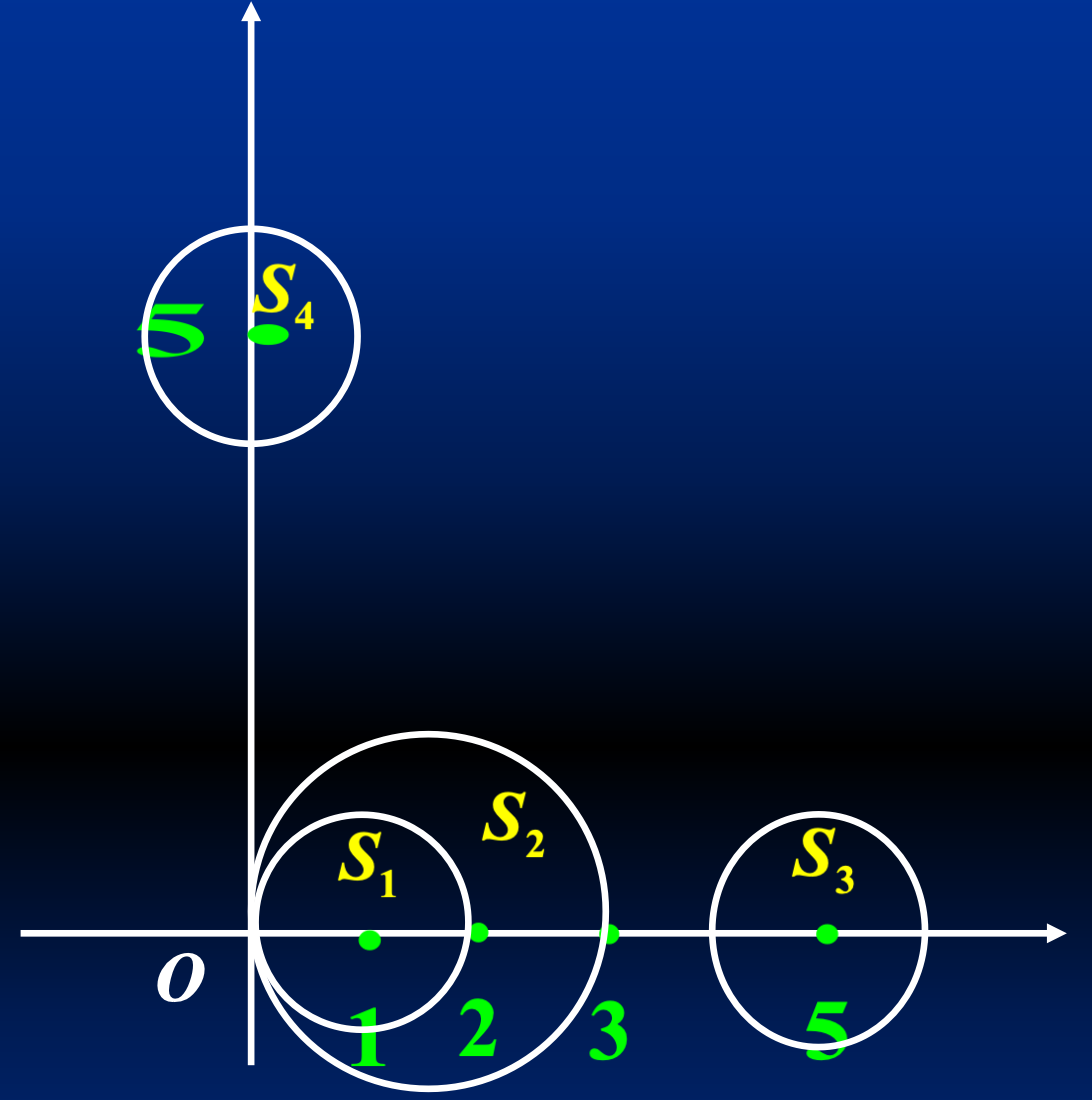
\includegraphics[scale=0.4]{盖尔圆1.png}
    \end{figure}

    这就是如何画出盖尔圆,这个矩阵的特征值就会分布在盖尔圆内。
\end{solution}

同样的,我们还有如下推论:
\begin{corollary}{}{}
    设$\A\in\C^{n\times n}$,则$\A$的任一特征值\[\lambda_i\in\bigcup_{j=1}^{n}G_i\]
\end{corollary}

也就是说,矩阵的特征值同样分布在列盖尔圆内。

\subsection{第二圆盘定理}
第一圆盘定理只说明了矩阵$\A$的特征值都在盖尔圆中,但并没有说哪个连通部分有哪些特征值,要让特征值的分布更明确,就需要第二圆盘定理。
\begin{them}{第二圆盘定理}{}
    设$n$阶方阵$\A$的$n$个盖尔圆盘中有$k$个圆盘的并形成一个连通区域$\G$,且它与余下的$n-k$个圆盘都不相交,则在该区域$\G$中恰好有$\A$的$k$个特征值。
\end{them}

这里仅仅解释一下何为“连通”,关于该定理的证明就不赘述了,详细可以看PPT或者课本。

以例\ref{exp:4.1.1}画出的盖尔圆为例,$S_1, S_2$重叠在一起,它们的并集是一个连通区域,交结在一起的盖尔圆所构成的连通区域为并集$S$的一个连通部分,孤立的盖尔圆就是一个连通部分,所以,$S_1$与$S_2$的并集,即$S_2$、$S_3\text{、}S_4$各是一个连通部分。

\subsection{圆盘定理的其他推论}
接下来介绍的圆盘定理的其他推论更有助于借助圆盘来判断矩阵特征值的情况:
\begin{corollary}{}{}
    设$n$阶方阵$\A$的$n$个盖尔圆盘两两互不相交,则$\A$相似于对角阵。
\end{corollary}
如果$n$个盖尔圆盘两两互不相交,则说明每一个盖尔圆盘就包含一个矩阵的特征值,这也就是说$n$个盖尔圆盘就会有$n$个互不相同的特征值,由线性代数的知识可知,矩阵$\A$可以相似对角化。
\begin{corollary}{}{}
    设$n$阶实矩阵$\A$的$n$个盖尔圆盘两两互不相交,则$\A$的特征值全为实数。
\end{corollary}
如果$\A$不是实数而是复数的话,圆盘里面会有两个特征值,这与第二圆盘定理相矛盾。
\subsection{缩小特征值的范围}
圆盘定理虽然可以帮助确定特征值的范围,但这个范围我们还可以通过一些处理进行缩小,这就要利用到下面在线性代数中学到的性质:对于一个矩阵$\A$,乘上一个可逆矩阵,不改变矩阵特征值。

对于一个矩阵$\A$,我们做出如下处理:左乘一个可逆矩阵$\bs{S}^{-1}$,右乘一个$\bs{S}$,于是,对下面的一个新的矩阵画盖尔圆盘:\[\bs{S}^{-1}\bs{A}\bs{S}\]

如果对于$\bs{S}$的选择较为恰当,是能够得到更精确的特征值范围的,通常,一个比较特别的选择是选取\[\bs{S}=\D=diag(p_1, p_2,\cdots,p_n)\ \ \ p_i>0\ (i=1,2,\cdots,n)\]这样的一个对角矩阵,于是,新的矩阵就成了
\[
\begin{aligned}
\bs{S}^{-1}\bs{A}\bs{S}&=\begin{bmatrix}
    p_1^{-1}&&&\\
    &p_2^{-1}&&\\
    &&\ddots &\\
    &&&p_4^{-1}
\end{bmatrix}\cdot
\begin{bmatrix}
    a_{11}&a_{12}&\cdots&a_{1n}\\
    a_{21}&a_{22}&\cdots&a_{2n}\\
    \vdots&\vdots&\vdots\\
    a_{n1}&a_{n2}&\cdots&a_{nn}
\end{bmatrix}\cdot
\begin{bmatrix}
    p_1&&&\\
    &p_2&&\\
    &&\ddots &\\
    &&&p_4
\end{bmatrix}\\
&=\begin{bmatrix}
    \frac{a_{11}}{p_1}&\frac{a_{12}}{p_1}&\cdots&\frac{a_{1n}}{p_1}\\
    \frac{a_{21}}{p_2}&\frac{a_{22}}{p_2}&\cdots&\frac{a_{2n}}{p_2}\\
    \vdots&\vdots&&\vdots\\
    \frac{a_{n1}}{p_n}&\frac{a_{n2}}{p_n}&\cdots&\frac{a_{nn}}{p_n}
\end{bmatrix}\cdot
\begin{bmatrix}
    p_1&&&\\
    &p_2&&\\
    &&\ddots &\\
    &&&p_4
\end{bmatrix}\\
&=\begin{bmatrix}
    a_{11}&\frac{p_2}{p_1}a_{12}&\cdots&\frac{p_n}{p_1}a_{1n}\\
    \frac{p_1}{p_2}a_{21}&a_{22}&\cdots&\frac{p_n}{p_2}a_{2n}\\
    \vdots&\vdots&&\vdots\\
    \frac{p_1}{p_n}a_{n1}&\frac{p_2}{p_n}a_{n2}&\cdots&a_{nn}
\end{bmatrix}
\end{aligned}
\]

这个时候下的盖尔圆的半径可以受$\bs{S}$矩阵的对角元素来影响,可以看到,以第一行为例,可以增大$p_1$的值,减小$p_2,\cdots,p_n$的值,这个时候盖尔圆$S_1$就会变小,可相对应的会发现,$S_2,\cdots,S_n$的半径就会变大。

采用这种方式和正常求盖尔圆的对于特征值影响到底有多大呢?请看下面的例子:
\begin{example}
    估计矩阵\[\A=\begin{bmatrix}
        0.9&0.01&0.12\\
        0.01&0.8&0.13\\
        0.01&0.02&0.4
    \end{bmatrix}\]的特征值的范围。
\end{example}
\begin{solution}
    
    如果采用原始方法,求解的盖尔圆的信息如下:
    \[S_1:|z-0.9|\leq0.13\]
    \[S_2:|z-0.8|\leq0.14\]
    \[S_3:|z-0.4|\leq0.03\]

    若取$p_1=p_2=1, p_3=0.1$,则\[\D=diag(1,1,0.1)\]
    新的盖尔圆盘信息就成了:
    \[S'_1:|z-0.9|\leq 0.022\]
    \[S'_2:|z-0.8|\leq 0.023\]
    \[S'_3:|z-0.4|\leq 0.3\]

    对比一下就会发现,前面两个盖尔圆盘($S_1, S_2$)的半径的确变小了,代表特征值的范围更加精确,但相对应的,$S_3$的半径变大,特征值的范围更加模糊。
\end{solution}

\subsection{盖尔圆盘的其他性质}

在本节的最后,介绍一下其他盖尔圆盘的性质
\subsubsection{行对角占优和列对角占优}
\begin{defn}{行对角占优和列对角占优}{}
    设$\a\in\C^{n\times n}$,则\begin{enumerate}
        \item 若$|a_{ii}|\geq R_i$,则称该矩阵为\textbf{行对角占优}。
        \item 若$|a_{ii}|\geq C_i$,则称该矩阵为\textbf{列对角占优}。
    \end{enumerate}
    如果去掉等于号,上面的两个就成了\textbf{行严格对角占优}和\textbf{列严格对角占优}。
\end{defn}

这两个概念是为了下面的定理服务的,这里不给出证明,感兴趣的可以自己翻课本
\begin{them}{}{}
    设$\A\in\C^{n\times n}$行(或列)严格对角占优,则\begin{enumerate}
        \item $\A$可逆,且$\lambda_i\in\bigcup_{i=1}^{n}S_i\ \ \ (S_i=\{z\in\C:|z-a_{ii}|\leq |a_{ii}|\})$
        \item 若$\A$的所有主对角元都为正数,则$\A$的特征值都有正实部
        \item 若$\A$为Hermite矩阵,且所有主对角元都为正数,则$\A$的特征值都为正数。
    \end{enumerate}
\end{them}
\ifx\allfiles\undefined
\end{document}
\fi